% =====================================================================
%  Laboratorio de la Sesión 4: GMM y k-medias en Iris
%  Se incluye desde Sesion4-GMM.tex con % =====================================================================
%  Laboratorio de la Sesión 4: GMM y k-medias en Iris
%  Se incluye desde Sesion4-GMM.tex con % =====================================================================
%  Laboratorio de la Sesión 4: GMM y k-medias en Iris
%  Se incluye desde Sesion4-GMM.tex con % =====================================================================
%  Laboratorio de la Sesión 4: GMM y k-medias en Iris
%  Se incluye desde Sesion4-GMM.tex con \input{Laboratorio}
%  El mismo código, ejecutado, está en laboratorio_gmm.ipynb
% =====================================================================
\section{Laboratorio: GMM y k-medias en Iris}
% =====================================================================

\begin{frame}[fragile]{Paso 1: ajustar la mezcla}
\begin{lstlisting}
import numpy as np, pandas as pd
from sklearn.datasets import load_iris
from sklearn.mixture import GaussianMixture
from sklearn.cluster import KMeans
from sklearn.metrics import adjusted_rand_score

X, especie = load_iris(return_X_y=True)     # la especie NO se usa para ajustar
gm = GaussianMixture(n_components=3, covariance_type="full", n_init=10, random_state=0).fit(X)
print(gm.converged_, gm.n_iter_, gm.weights_.round(2))
z = gm.predict(X)
print(pd.crosstab(z, especie), adjusted_rand_score(especie, z))
\end{lstlisting}
  \begin{columns}[T]
    \column{0.5\textwidth}
    \small
    \begin{itemize}
      \item EM converge en 17 iteraciones.
      \item Pesos: 0.30, 0.33 y 0.37.
      \item Índice de Rand ajustado contra la especie: \textbf{0.90}
            (k-medias obtuvo 0.73 en la Sesión 2).
    \end{itemize}
    \column{0.45\textwidth}
    \small
    \centering
    \begin{tabular}{@{}lccc@{}}
      & \textbf{setosa} & \textbf{versic.} & \textbf{virgin.}\\
      \midrule
      Comp. 1 & 0 & 45 & 0 \\
      Comp. 2 & 50 & 0 & 0 \\
      Comp. 3 & 0 & 5 & 50 \\
    \end{tabular}
  \end{columns}
\end{frame}

\begin{frame}[fragile]{Paso 2: asignaciones suaves}
\begin{lstlisting}
P = gm.predict_proba(X)                     # 150 x 3, cada fila suma 1
inciertas = np.where(P.max(axis=1) < 0.9)[0]
print((P.max(axis=1) > 0.99).sum(), inciertas, P[inciertas].round(2))
\end{lstlisting}
  \small
  \begin{itemize}
    \item 132 de las 150 flores tienen una probabilidad mayor que 0.99 en su componente.
    \item Sólo 3 tienen probabilidad máxima menor que 0.9:
  \end{itemize}
  \centering
  \begin{tabular}{@{}cccccc@{}}
    \toprule
    \textbf{Flor} & \textbf{Especie} & \textbf{Pétalo (cm)} & \textbf{P(comp. 1)} & \textbf{P(comp. 3)} & \textbf{Asignada a}\\
    \midrule
    77  & versicolor & $5.0 \times 1.7$ & 0.37 & 0.63 & comp. 3 (error) \\
    84  & versicolor & $4.5 \times 1.5$ & 0.86 & 0.14 & comp. 1 \\
    133 & virginica  & $5.1 \times 1.5$ & 0.24 & 0.76 & comp. 3 \\
    \bottomrule
  \end{tabular}
  \begin{itemize}
    \item Las tres están en la frontera entre versicolor y virginica: el modelo
          señala dónde puede equivocarse, cosa que k-medias no hace.
  \end{itemize}
\end{frame}

\begin{frame}[fragile]{Paso 3: comparar los tipos de covarianza}
\begin{lstlisting}
for tipo in ["full", "tied", "diag", "spherical"]:
    g = GaussianMixture(3, covariance_type=tipo, n_init=10, random_state=0).fit(X)
    z = g.predict(X)
    print(tipo, g._n_parameters(), round(g.bic(X), 1),
          round(adjusted_rand_score(especie, z), 2), np.bincount(z))
\end{lstlisting}
  \begin{columns}[c]
    \column{0.5\textwidth}
    \small
    \centering
    \begin{tabular}{@{}lccc@{}}
      \toprule
      \textbf{Tipo} & \textbf{Parám.} & \textbf{BIC} & \textbf{ARI}\\
      \midrule
      \texttt{full}      & 44 & 580.9 & 0.90 \\
      \texttt{tied}      & 24 & 633.8 & 0.89 \\
      \texttt{diag}      & 26 & 744.6 & 0.76 \\
      \texttt{spherical} & 17 & 853.8 & 0.73 \\
      \bottomrule
    \end{tabular}
    \column{0.48\textwidth}
    \small
    \begin{itemize}
      \item Los grupos de Iris son elipses inclinadas: las medidas de una flor están correlacionadas.
      \item \texttt{full} y \texttt{tied} las capturan.
      \item \texttt{spherical} obtiene el mismo ARI que k-medias (0.73).
      \item BIC ordena los tipos igual que el ARI, sin usar las especies.
    \end{itemize}
  \end{columns}
\end{frame}

\begin{frame}[fragile]{Paso 4: elegir $K$ con BIC y AIC}
\begin{lstlisting}
for tipo in ["full", "tied", "diag", "spherical"]:
    for k in range(1, 7):
        g = GaussianMixture(k, covariance_type=tipo, n_init=10, random_state=0).fit(X)
        print(tipo, k, round(g.bic(X), 1), round(g.aic(X), 1))
\end{lstlisting}
  \begin{columns}[c]
    \column{0.55\textwidth}
    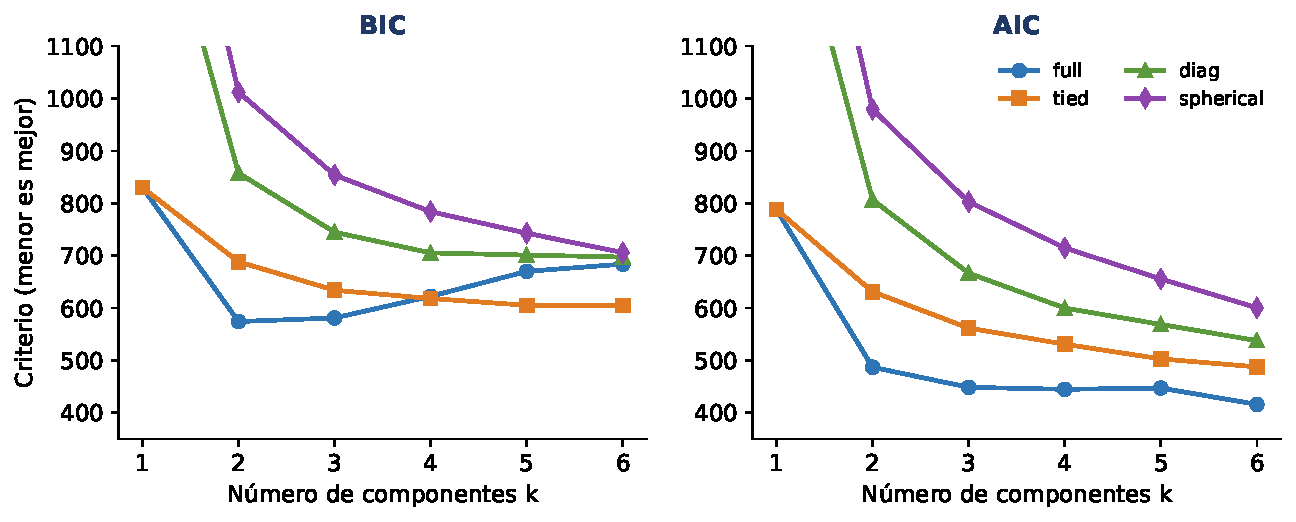
\includegraphics[width=\textwidth]{iris_bic}
    \column{0.43\textwidth}
    \small
    \begin{itemize}
      \item BIC más bajo: \texttt{full} con $K=2$ (574.0); $K=3$ queda muy cerca (580.9).
      \item Otra vez las dos escalas de Iris: setosa contra el resto, y después
            versicolor contra virginica.
      \item AIC sigue bajando con \texttt{full} hasta $K=6$ (415.7): penaliza menos y elige más
            componentes.
    \end{itemize}
  \end{columns}
\end{frame}

\begin{frame}[fragile]{Paso 5: GMM contra k-medias}
\begin{lstlisting}
z_km = KMeans(n_clusters=3, n_init=10, random_state=0).fit_predict(X)
print(pd.crosstab(z_km, especie), adjusted_rand_score(especie, z_km))
\end{lstlisting}
  \centering
  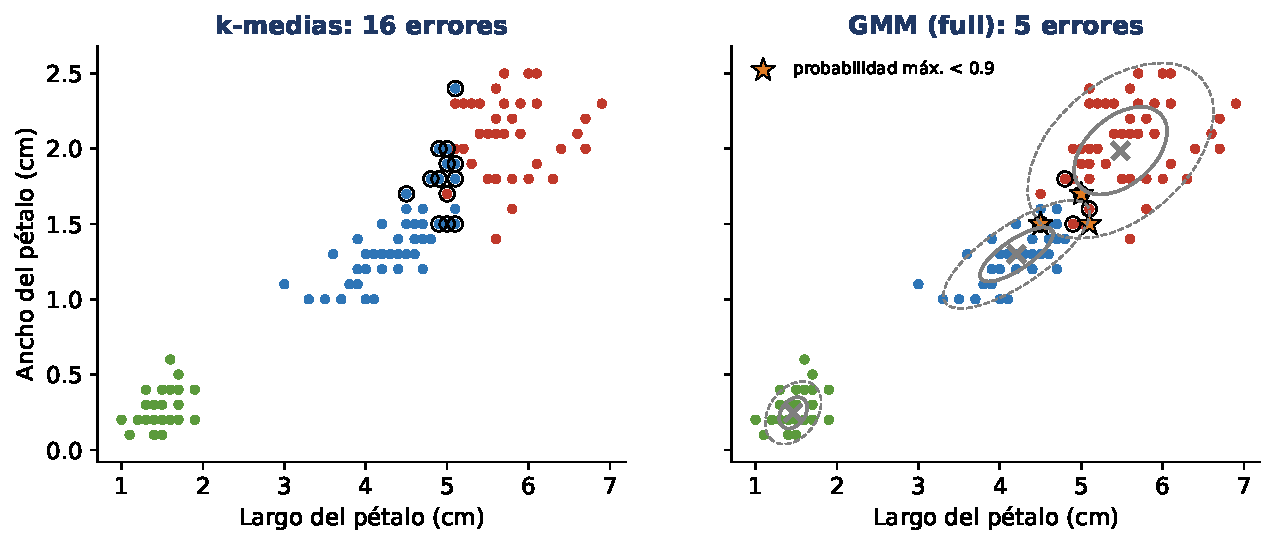
\includegraphics[width=0.66\textwidth]{iris_gmm}
  \small
  \begin{itemize}
    \item k-medias: 16 flores fuera de su especie (14 virginica con versicolor y 2 al revés);
          GMM: 5, todas versicolor. Círculos: errores; estrellas: flores inciertas.
    \item La elipse de virginica es más grande e inclinada; k-medias corta a la mitad entre los centros.
  \end{itemize}
\end{frame}

\begin{frame}{Conclusiones del laboratorio}
  \begin{itemize}
    \item Con covarianza completa, la mezcla gaussiana se acerca más a las especies que
          k-medias (ARI 0.90 contra 0.73) porque los grupos de Iris son elípticos.
    \item Las probabilidades indican qué flores están en la frontera; las 3 flores inciertas
          son de versicolor y virginica.
    \item El tipo de covarianza importa: \texttt{spherical} se comporta como k-medias.
    \item BIC elige el tipo de covarianza correcto sin usar etiquetas; para $K$ duda entre 2 y 3,
          igual que la silueta y el dendrograma en las sesiones anteriores.
    \item AIC elige demasiados componentes cuando el objetivo es contar grupos.
  \end{itemize}
\end{frame}

%  El mismo código, ejecutado, está en laboratorio_gmm.ipynb
% =====================================================================
\section{Laboratorio: GMM y k-medias en Iris}
% =====================================================================

\begin{frame}[fragile]{Paso 1: ajustar la mezcla}
\begin{lstlisting}
import numpy as np, pandas as pd
from sklearn.datasets import load_iris
from sklearn.mixture import GaussianMixture
from sklearn.cluster import KMeans
from sklearn.metrics import adjusted_rand_score

X, especie = load_iris(return_X_y=True)     # la especie NO se usa para ajustar
gm = GaussianMixture(n_components=3, covariance_type="full", n_init=10, random_state=0).fit(X)
print(gm.converged_, gm.n_iter_, gm.weights_.round(2))
z = gm.predict(X)
print(pd.crosstab(z, especie), adjusted_rand_score(especie, z))
\end{lstlisting}
  \begin{columns}[T]
    \column{0.5\textwidth}
    \small
    \begin{itemize}
      \item EM converge en 17 iteraciones.
      \item Pesos: 0.30, 0.33 y 0.37.
      \item Índice de Rand ajustado contra la especie: \textbf{0.90}
            (k-medias obtuvo 0.73 en la Sesión 2).
    \end{itemize}
    \column{0.45\textwidth}
    \small
    \centering
    \begin{tabular}{@{}lccc@{}}
      & \textbf{setosa} & \textbf{versic.} & \textbf{virgin.}\\
      \midrule
      Comp. 1 & 0 & 45 & 0 \\
      Comp. 2 & 50 & 0 & 0 \\
      Comp. 3 & 0 & 5 & 50 \\
    \end{tabular}
  \end{columns}
\end{frame}

\begin{frame}[fragile]{Paso 2: asignaciones suaves}
\begin{lstlisting}
P = gm.predict_proba(X)                     # 150 x 3, cada fila suma 1
inciertas = np.where(P.max(axis=1) < 0.9)[0]
print((P.max(axis=1) > 0.99).sum(), inciertas, P[inciertas].round(2))
\end{lstlisting}
  \small
  \begin{itemize}
    \item 132 de las 150 flores tienen una probabilidad mayor que 0.99 en su componente.
    \item Sólo 3 tienen probabilidad máxima menor que 0.9:
  \end{itemize}
  \centering
  \begin{tabular}{@{}cccccc@{}}
    \toprule
    \textbf{Flor} & \textbf{Especie} & \textbf{Pétalo (cm)} & \textbf{P(comp. 1)} & \textbf{P(comp. 3)} & \textbf{Asignada a}\\
    \midrule
    77  & versicolor & $5.0 \times 1.7$ & 0.37 & 0.63 & comp. 3 (error) \\
    84  & versicolor & $4.5 \times 1.5$ & 0.86 & 0.14 & comp. 1 \\
    133 & virginica  & $5.1 \times 1.5$ & 0.24 & 0.76 & comp. 3 \\
    \bottomrule
  \end{tabular}
  \begin{itemize}
    \item Las tres están en la frontera entre versicolor y virginica: el modelo
          señala dónde puede equivocarse, cosa que k-medias no hace.
  \end{itemize}
\end{frame}

\begin{frame}[fragile]{Paso 3: comparar los tipos de covarianza}
\begin{lstlisting}
for tipo in ["full", "tied", "diag", "spherical"]:
    g = GaussianMixture(3, covariance_type=tipo, n_init=10, random_state=0).fit(X)
    z = g.predict(X)
    print(tipo, g._n_parameters(), round(g.bic(X), 1),
          round(adjusted_rand_score(especie, z), 2), np.bincount(z))
\end{lstlisting}
  \begin{columns}[c]
    \column{0.5\textwidth}
    \small
    \centering
    \begin{tabular}{@{}lccc@{}}
      \toprule
      \textbf{Tipo} & \textbf{Parám.} & \textbf{BIC} & \textbf{ARI}\\
      \midrule
      \texttt{full}      & 44 & 580.9 & 0.90 \\
      \texttt{tied}      & 24 & 633.8 & 0.89 \\
      \texttt{diag}      & 26 & 744.6 & 0.76 \\
      \texttt{spherical} & 17 & 853.8 & 0.73 \\
      \bottomrule
    \end{tabular}
    \column{0.48\textwidth}
    \small
    \begin{itemize}
      \item Los grupos de Iris son elipses inclinadas: las medidas de una flor están correlacionadas.
      \item \texttt{full} y \texttt{tied} las capturan.
      \item \texttt{spherical} obtiene el mismo ARI que k-medias (0.73).
      \item BIC ordena los tipos igual que el ARI, sin usar las especies.
    \end{itemize}
  \end{columns}
\end{frame}

\begin{frame}[fragile]{Paso 4: elegir $K$ con BIC y AIC}
\begin{lstlisting}
for tipo in ["full", "tied", "diag", "spherical"]:
    for k in range(1, 7):
        g = GaussianMixture(k, covariance_type=tipo, n_init=10, random_state=0).fit(X)
        print(tipo, k, round(g.bic(X), 1), round(g.aic(X), 1))
\end{lstlisting}
  \begin{columns}[c]
    \column{0.55\textwidth}
    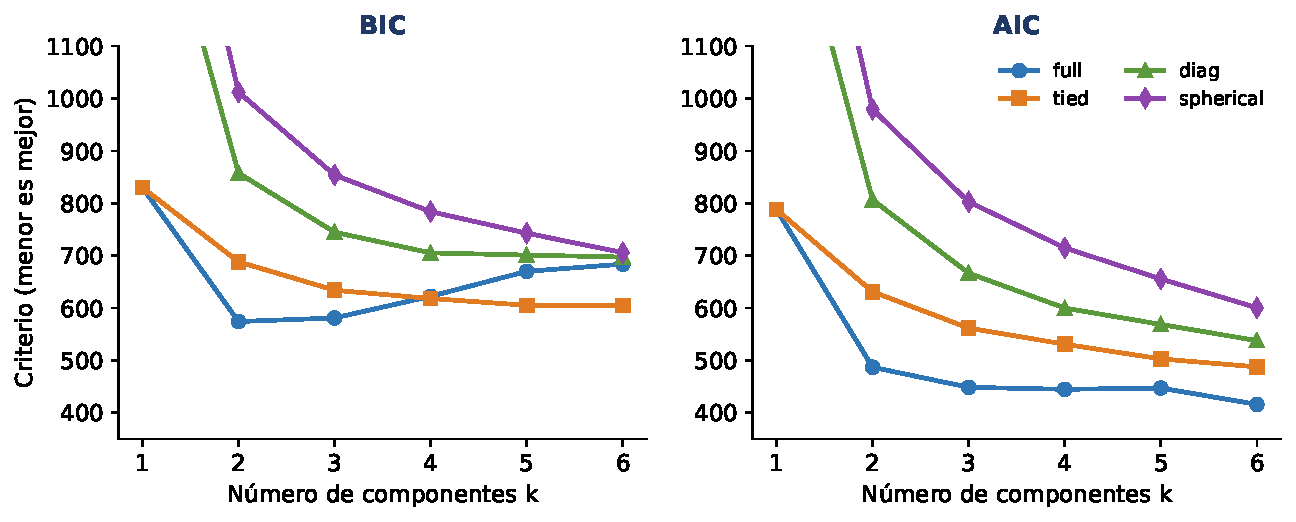
\includegraphics[width=\textwidth]{iris_bic}
    \column{0.43\textwidth}
    \small
    \begin{itemize}
      \item BIC más bajo: \texttt{full} con $K=2$ (574.0); $K=3$ queda muy cerca (580.9).
      \item Otra vez las dos escalas de Iris: setosa contra el resto, y después
            versicolor contra virginica.
      \item AIC sigue bajando con \texttt{full} hasta $K=6$ (415.7): penaliza menos y elige más
            componentes.
    \end{itemize}
  \end{columns}
\end{frame}

\begin{frame}[fragile]{Paso 5: GMM contra k-medias}
\begin{lstlisting}
z_km = KMeans(n_clusters=3, n_init=10, random_state=0).fit_predict(X)
print(pd.crosstab(z_km, especie), adjusted_rand_score(especie, z_km))
\end{lstlisting}
  \centering
  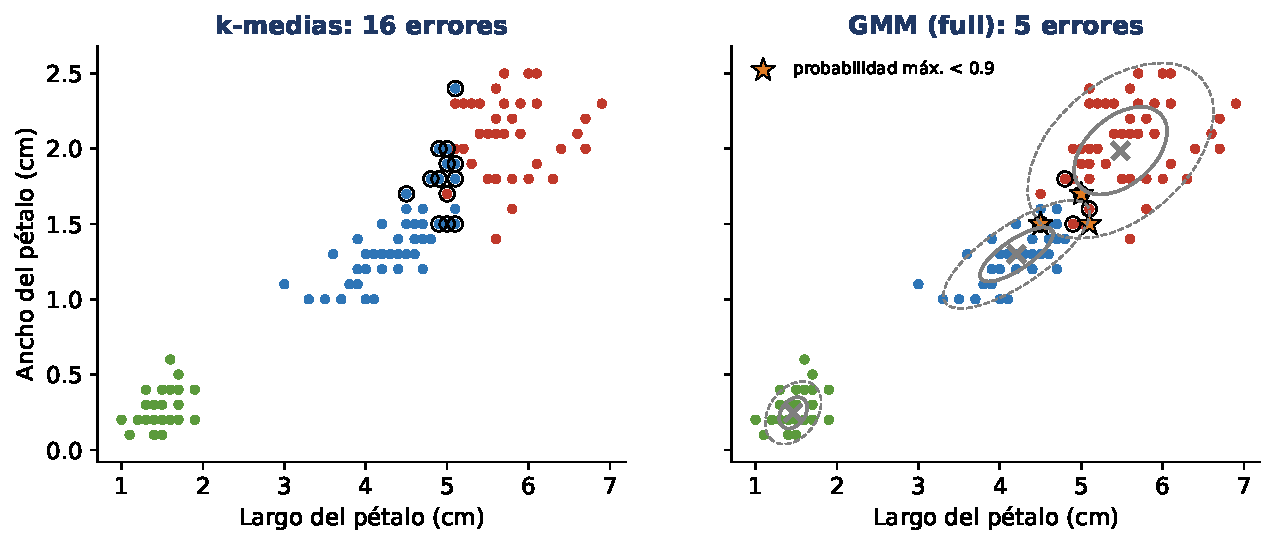
\includegraphics[width=0.66\textwidth]{iris_gmm}
  \small
  \begin{itemize}
    \item k-medias: 16 flores fuera de su especie (14 virginica con versicolor y 2 al revés);
          GMM: 5, todas versicolor. Círculos: errores; estrellas: flores inciertas.
    \item La elipse de virginica es más grande e inclinada; k-medias corta a la mitad entre los centros.
  \end{itemize}
\end{frame}

\begin{frame}{Conclusiones del laboratorio}
  \begin{itemize}
    \item Con covarianza completa, la mezcla gaussiana se acerca más a las especies que
          k-medias (ARI 0.90 contra 0.73) porque los grupos de Iris son elípticos.
    \item Las probabilidades indican qué flores están en la frontera; las 3 flores inciertas
          son de versicolor y virginica.
    \item El tipo de covarianza importa: \texttt{spherical} se comporta como k-medias.
    \item BIC elige el tipo de covarianza correcto sin usar etiquetas; para $K$ duda entre 2 y 3,
          igual que la silueta y el dendrograma en las sesiones anteriores.
    \item AIC elige demasiados componentes cuando el objetivo es contar grupos.
  \end{itemize}
\end{frame}

%  El mismo código, ejecutado, está en laboratorio_gmm.ipynb
% =====================================================================
\section{Laboratorio: GMM y k-medias en Iris}
% =====================================================================

\begin{frame}[fragile]{Paso 1: ajustar la mezcla}
\begin{lstlisting}
import numpy as np, pandas as pd
from sklearn.datasets import load_iris
from sklearn.mixture import GaussianMixture
from sklearn.cluster import KMeans
from sklearn.metrics import adjusted_rand_score

X, especie = load_iris(return_X_y=True)     # la especie NO se usa para ajustar
gm = GaussianMixture(n_components=3, covariance_type="full", n_init=10, random_state=0).fit(X)
print(gm.converged_, gm.n_iter_, gm.weights_.round(2))
z = gm.predict(X)
print(pd.crosstab(z, especie), adjusted_rand_score(especie, z))
\end{lstlisting}
  \begin{columns}[T]
    \column{0.5\textwidth}
    \small
    \begin{itemize}
      \item EM converge en 17 iteraciones.
      \item Pesos: 0.30, 0.33 y 0.37.
      \item Índice de Rand ajustado contra la especie: \textbf{0.90}
            (k-medias obtuvo 0.73 en la Sesión 2).
    \end{itemize}
    \column{0.45\textwidth}
    \small
    \centering
    \begin{tabular}{@{}lccc@{}}
      & \textbf{setosa} & \textbf{versic.} & \textbf{virgin.}\\
      \midrule
      Comp. 1 & 0 & 45 & 0 \\
      Comp. 2 & 50 & 0 & 0 \\
      Comp. 3 & 0 & 5 & 50 \\
    \end{tabular}
  \end{columns}
\end{frame}

\begin{frame}[fragile]{Paso 2: asignaciones suaves}
\begin{lstlisting}
P = gm.predict_proba(X)                     # 150 x 3, cada fila suma 1
inciertas = np.where(P.max(axis=1) < 0.9)[0]
print((P.max(axis=1) > 0.99).sum(), inciertas, P[inciertas].round(2))
\end{lstlisting}
  \small
  \begin{itemize}
    \item 132 de las 150 flores tienen una probabilidad mayor que 0.99 en su componente.
    \item Sólo 3 tienen probabilidad máxima menor que 0.9:
  \end{itemize}
  \centering
  \begin{tabular}{@{}cccccc@{}}
    \toprule
    \textbf{Flor} & \textbf{Especie} & \textbf{Pétalo (cm)} & \textbf{P(comp. 1)} & \textbf{P(comp. 3)} & \textbf{Asignada a}\\
    \midrule
    77  & versicolor & $5.0 \times 1.7$ & 0.37 & 0.63 & comp. 3 (error) \\
    84  & versicolor & $4.5 \times 1.5$ & 0.86 & 0.14 & comp. 1 \\
    133 & virginica  & $5.1 \times 1.5$ & 0.24 & 0.76 & comp. 3 \\
    \bottomrule
  \end{tabular}
  \begin{itemize}
    \item Las tres están en la frontera entre versicolor y virginica: el modelo
          señala dónde puede equivocarse, cosa que k-medias no hace.
  \end{itemize}
\end{frame}

\begin{frame}[fragile]{Paso 3: comparar los tipos de covarianza}
\begin{lstlisting}
for tipo in ["full", "tied", "diag", "spherical"]:
    g = GaussianMixture(3, covariance_type=tipo, n_init=10, random_state=0).fit(X)
    z = g.predict(X)
    print(tipo, g._n_parameters(), round(g.bic(X), 1),
          round(adjusted_rand_score(especie, z), 2), np.bincount(z))
\end{lstlisting}
  \begin{columns}[c]
    \column{0.5\textwidth}
    \small
    \centering
    \begin{tabular}{@{}lccc@{}}
      \toprule
      \textbf{Tipo} & \textbf{Parám.} & \textbf{BIC} & \textbf{ARI}\\
      \midrule
      \texttt{full}      & 44 & 580.9 & 0.90 \\
      \texttt{tied}      & 24 & 633.8 & 0.89 \\
      \texttt{diag}      & 26 & 744.6 & 0.76 \\
      \texttt{spherical} & 17 & 853.8 & 0.73 \\
      \bottomrule
    \end{tabular}
    \column{0.48\textwidth}
    \small
    \begin{itemize}
      \item Los grupos de Iris son elipses inclinadas: las medidas de una flor están correlacionadas.
      \item \texttt{full} y \texttt{tied} las capturan.
      \item \texttt{spherical} obtiene el mismo ARI que k-medias (0.73).
      \item BIC ordena los tipos igual que el ARI, sin usar las especies.
    \end{itemize}
  \end{columns}
\end{frame}

\begin{frame}[fragile]{Paso 4: elegir $K$ con BIC y AIC}
\begin{lstlisting}
for tipo in ["full", "tied", "diag", "spherical"]:
    for k in range(1, 7):
        g = GaussianMixture(k, covariance_type=tipo, n_init=10, random_state=0).fit(X)
        print(tipo, k, round(g.bic(X), 1), round(g.aic(X), 1))
\end{lstlisting}
  \begin{columns}[c]
    \column{0.55\textwidth}
    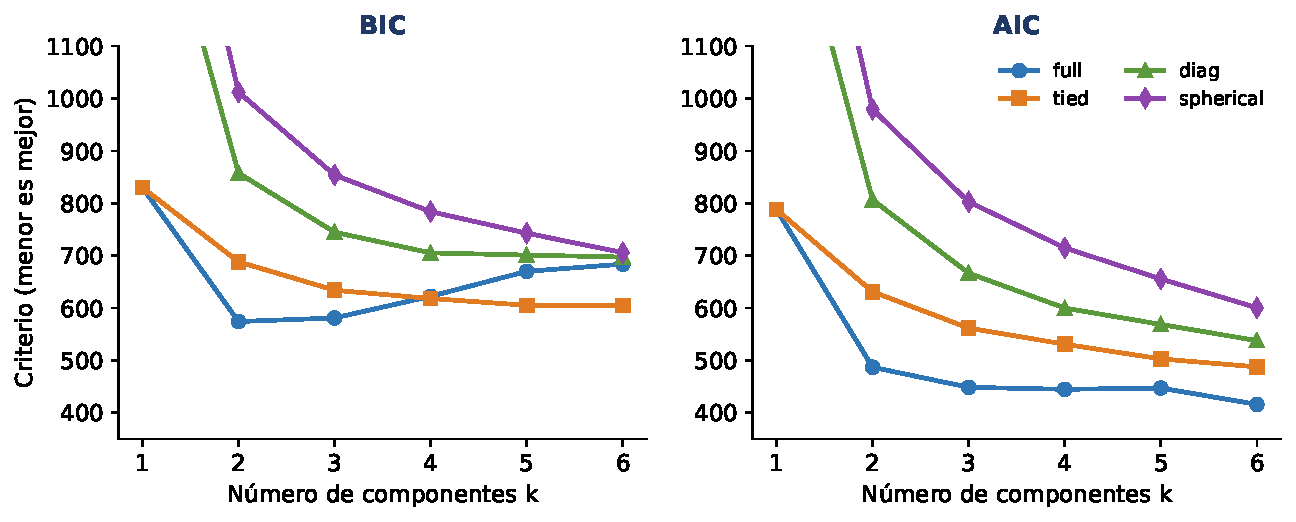
\includegraphics[width=\textwidth]{iris_bic}
    \column{0.43\textwidth}
    \small
    \begin{itemize}
      \item BIC más bajo: \texttt{full} con $K=2$ (574.0); $K=3$ queda muy cerca (580.9).
      \item Otra vez las dos escalas de Iris: setosa contra el resto, y después
            versicolor contra virginica.
      \item AIC sigue bajando con \texttt{full} hasta $K=6$ (415.7): penaliza menos y elige más
            componentes.
    \end{itemize}
  \end{columns}
\end{frame}

\begin{frame}[fragile]{Paso 5: GMM contra k-medias}
\begin{lstlisting}
z_km = KMeans(n_clusters=3, n_init=10, random_state=0).fit_predict(X)
print(pd.crosstab(z_km, especie), adjusted_rand_score(especie, z_km))
\end{lstlisting}
  \centering
  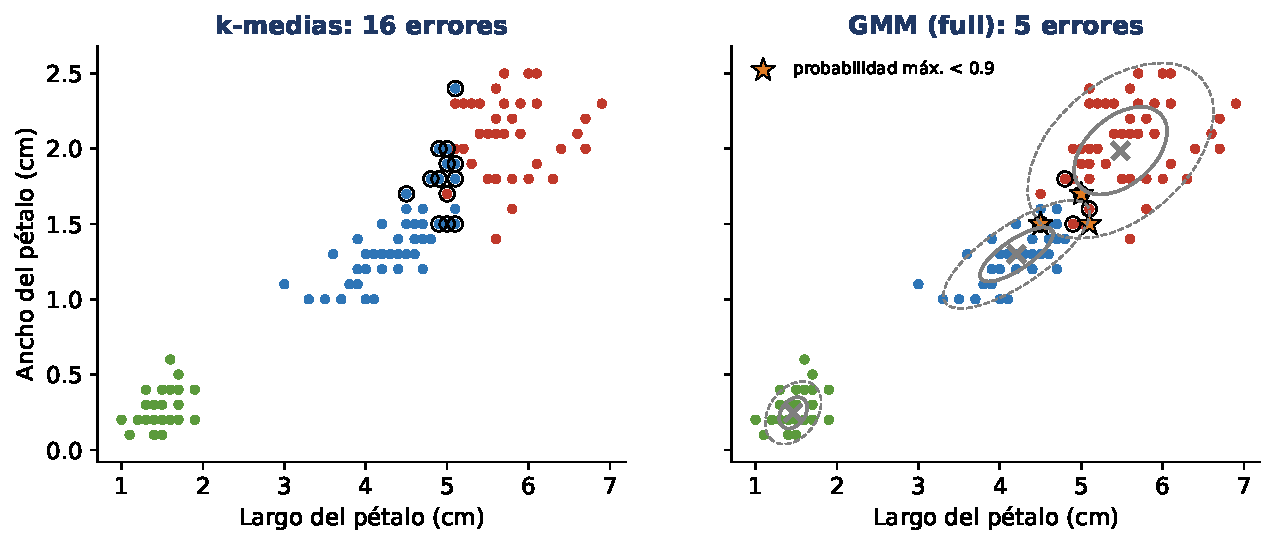
\includegraphics[width=0.66\textwidth]{iris_gmm}
  \small
  \begin{itemize}
    \item k-medias: 16 flores fuera de su especie (14 virginica con versicolor y 2 al revés);
          GMM: 5, todas versicolor. Círculos: errores; estrellas: flores inciertas.
    \item La elipse de virginica es más grande e inclinada; k-medias corta a la mitad entre los centros.
  \end{itemize}
\end{frame}

\begin{frame}{Conclusiones del laboratorio}
  \begin{itemize}
    \item Con covarianza completa, la mezcla gaussiana se acerca más a las especies que
          k-medias (ARI 0.90 contra 0.73) porque los grupos de Iris son elípticos.
    \item Las probabilidades indican qué flores están en la frontera; las 3 flores inciertas
          son de versicolor y virginica.
    \item El tipo de covarianza importa: \texttt{spherical} se comporta como k-medias.
    \item BIC elige el tipo de covarianza correcto sin usar etiquetas; para $K$ duda entre 2 y 3,
          igual que la silueta y el dendrograma en las sesiones anteriores.
    \item AIC elige demasiados componentes cuando el objetivo es contar grupos.
  \end{itemize}
\end{frame}

%  El mismo código, ejecutado, está en laboratorio_gmm.ipynb
% =====================================================================
\section{Laboratorio: GMM y k-medias en Iris}
% =====================================================================

\begin{frame}[fragile]{Paso 1: ajustar la mezcla}
\begin{lstlisting}
import numpy as np, pandas as pd
from sklearn.datasets import load_iris
from sklearn.mixture import GaussianMixture
from sklearn.cluster import KMeans
from sklearn.metrics import adjusted_rand_score

X, especie = load_iris(return_X_y=True)     # la especie NO se usa para ajustar
gm = GaussianMixture(n_components=3, covariance_type="full", n_init=10, random_state=0).fit(X)
print(gm.converged_, gm.n_iter_, gm.weights_.round(2))
z = gm.predict(X)
print(pd.crosstab(z, especie), adjusted_rand_score(especie, z))
\end{lstlisting}
  \begin{columns}[T]
    \column{0.5\textwidth}
    \small
    \begin{itemize}
      \item EM converge en 17 iteraciones.
      \item Pesos: 0.30, 0.33 y 0.37.
      \item Índice de Rand ajustado contra la especie: \textbf{0.90}
            (k-medias obtuvo 0.73 en la Sesión 2).
    \end{itemize}
    \column{0.45\textwidth}
    \small
    \centering
    \begin{tabular}{@{}lccc@{}}
      & \textbf{setosa} & \textbf{versic.} & \textbf{virgin.}\\
      \midrule
      Comp. 1 & 0 & 45 & 0 \\
      Comp. 2 & 50 & 0 & 0 \\
      Comp. 3 & 0 & 5 & 50 \\
    \end{tabular}
  \end{columns}
\end{frame}

\begin{frame}[fragile]{Paso 2: asignaciones suaves}
\begin{lstlisting}
P = gm.predict_proba(X)                     # 150 x 3, cada fila suma 1
inciertas = np.where(P.max(axis=1) < 0.9)[0]
print((P.max(axis=1) > 0.99).sum(), inciertas, P[inciertas].round(2))
\end{lstlisting}
  \small
  \begin{itemize}
    \item 132 de las 150 flores tienen una probabilidad mayor que 0.99 en su componente.
    \item Sólo 3 tienen probabilidad máxima menor que 0.9:
  \end{itemize}
  \centering
  \begin{tabular}{@{}cccccc@{}}
    \toprule
    \textbf{Flor} & \textbf{Especie} & \textbf{Pétalo (cm)} & \textbf{P(comp. 1)} & \textbf{P(comp. 3)} & \textbf{Asignada a}\\
    \midrule
    77  & versicolor & $5.0 \times 1.7$ & 0.37 & 0.63 & comp. 3 (error) \\
    84  & versicolor & $4.5 \times 1.5$ & 0.86 & 0.14 & comp. 1 \\
    133 & virginica  & $5.1 \times 1.5$ & 0.24 & 0.76 & comp. 3 \\
    \bottomrule
  \end{tabular}
  \begin{itemize}
    \item Las tres están en la frontera entre versicolor y virginica: el modelo
          señala dónde puede equivocarse, cosa que k-medias no hace.
  \end{itemize}
\end{frame}

\begin{frame}[fragile]{Paso 3: comparar los tipos de covarianza}
\begin{lstlisting}
for tipo in ["full", "tied", "diag", "spherical"]:
    g = GaussianMixture(3, covariance_type=tipo, n_init=10, random_state=0).fit(X)
    z = g.predict(X)
    print(tipo, g._n_parameters(), round(g.bic(X), 1),
          round(adjusted_rand_score(especie, z), 2), np.bincount(z))
\end{lstlisting}
  \begin{columns}[c]
    \column{0.5\textwidth}
    \small
    \centering
    \begin{tabular}{@{}lccc@{}}
      \toprule
      \textbf{Tipo} & \textbf{Parám.} & \textbf{BIC} & \textbf{ARI}\\
      \midrule
      \texttt{full}      & 44 & 580.9 & 0.90 \\
      \texttt{tied}      & 24 & 633.8 & 0.89 \\
      \texttt{diag}      & 26 & 744.6 & 0.76 \\
      \texttt{spherical} & 17 & 853.8 & 0.73 \\
      \bottomrule
    \end{tabular}
    \column{0.48\textwidth}
    \small
    \begin{itemize}
      \item Los grupos de Iris son elipses inclinadas: las medidas de una flor están correlacionadas.
      \item \texttt{full} y \texttt{tied} las capturan.
      \item \texttt{spherical} obtiene el mismo ARI que k-medias (0.73).
      \item BIC ordena los tipos igual que el ARI, sin usar las especies.
    \end{itemize}
  \end{columns}
\end{frame}

\begin{frame}[fragile]{Paso 4: elegir $K$ con BIC y AIC}
\begin{lstlisting}
for tipo in ["full", "tied", "diag", "spherical"]:
    for k in range(1, 7):
        g = GaussianMixture(k, covariance_type=tipo, n_init=10, random_state=0).fit(X)
        print(tipo, k, round(g.bic(X), 1), round(g.aic(X), 1))
\end{lstlisting}
  \begin{columns}[c]
    \column{0.55\textwidth}
    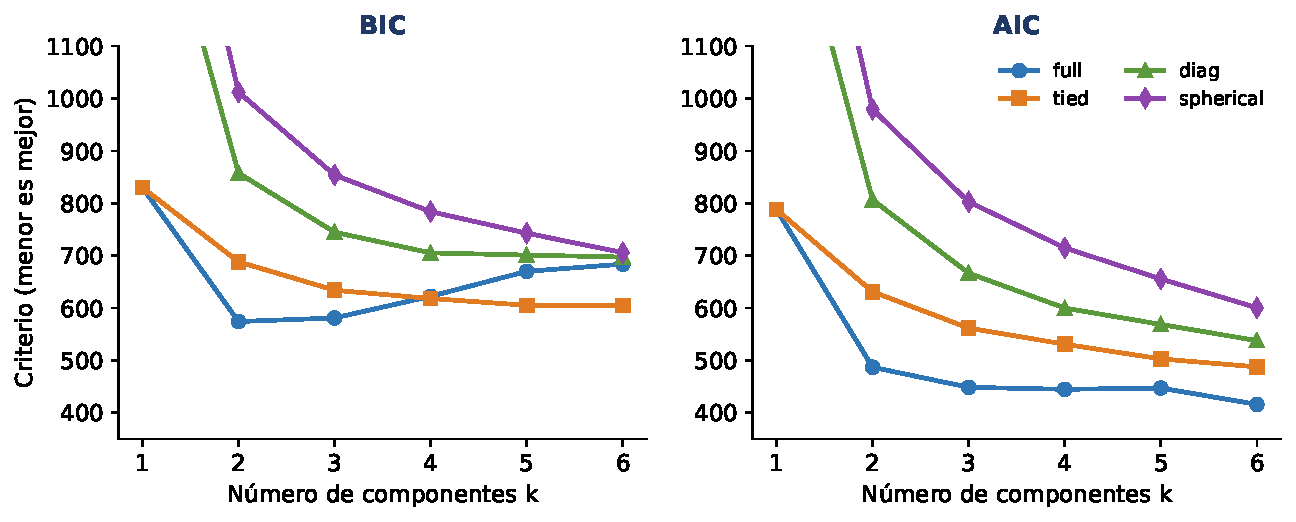
\includegraphics[width=\textwidth]{iris_bic}
    \column{0.43\textwidth}
    \small
    \begin{itemize}
      \item BIC más bajo: \texttt{full} con $K=2$ (574.0); $K=3$ queda muy cerca (580.9).
      \item Otra vez las dos escalas de Iris: setosa contra el resto, y después
            versicolor contra virginica.
      \item AIC sigue bajando con \texttt{full} hasta $K=6$ (415.7): penaliza menos y elige más
            componentes.
    \end{itemize}
  \end{columns}
\end{frame}

\begin{frame}[fragile]{Paso 5: GMM contra k-medias}
\begin{lstlisting}
z_km = KMeans(n_clusters=3, n_init=10, random_state=0).fit_predict(X)
print(pd.crosstab(z_km, especie), adjusted_rand_score(especie, z_km))
\end{lstlisting}
  \centering
  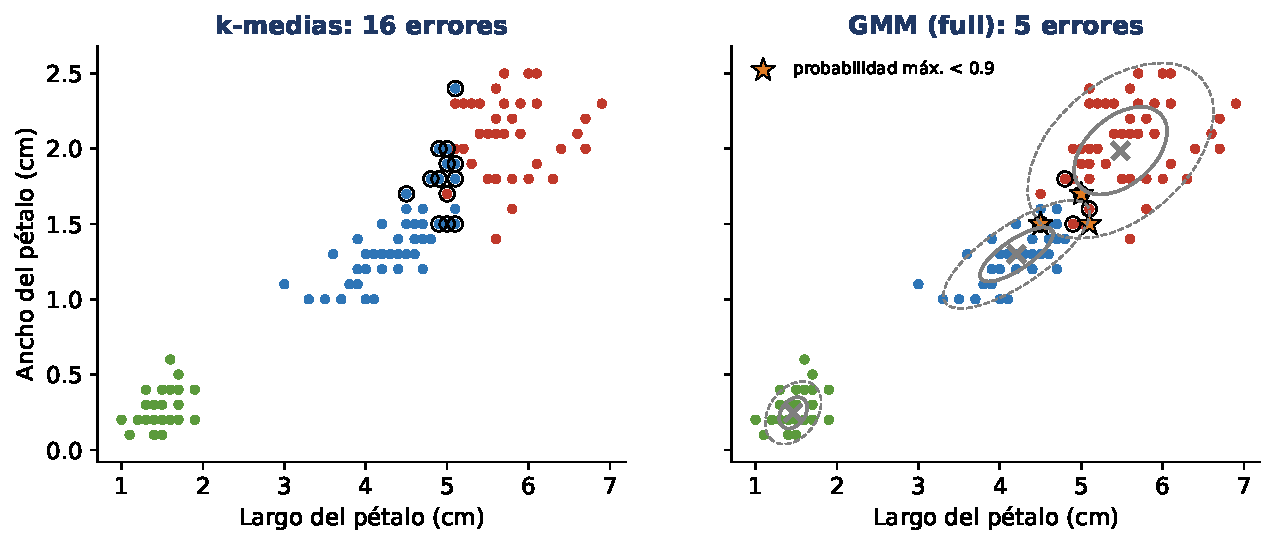
\includegraphics[width=0.66\textwidth]{iris_gmm}
  \small
  \begin{itemize}
    \item k-medias: 16 flores fuera de su especie (14 virginica con versicolor y 2 al revés);
          GMM: 5, todas versicolor. Círculos: errores; estrellas: flores inciertas.
    \item La elipse de virginica es más grande e inclinada; k-medias corta a la mitad entre los centros.
  \end{itemize}
\end{frame}

\begin{frame}{Conclusiones del laboratorio}
  \begin{itemize}
    \item Con covarianza completa, la mezcla gaussiana se acerca más a las especies que
          k-medias (ARI 0.90 contra 0.73) porque los grupos de Iris son elípticos.
    \item Las probabilidades indican qué flores están en la frontera; las 3 flores inciertas
          son de versicolor y virginica.
    \item El tipo de covarianza importa: \texttt{spherical} se comporta como k-medias.
    \item BIC elige el tipo de covarianza correcto sin usar etiquetas; para $K$ duda entre 2 y 3,
          igual que la silueta y el dendrograma en las sesiones anteriores.
    \item AIC elige demasiados componentes cuando el objetivo es contar grupos.
  \end{itemize}
\end{frame}
